
%--------------------------------------
\section{Modelling reactions}
%--------------------------------------

%----------------------------------
%\subsection{Some scattering theory}

\slide{}
\begin{center}
\psframebox[fillcolor=green!10,linecolor=blue,framearc=0.1,fillstyle=solid,framesep=5pt]{
Modelling nuclear reactions
}%psframe
\end{center} 
\end{frame}


%-----------------------------------------------------------------------------------------
\slide{Why reaction theory is important?}

\begin{itemize}
\setlength{\itemsep}{14pt}
\item Reaction theory provides the necessary framework to extract meaningful {\blue structure} information from measured {\blue cross sections} and also permits the understanding of the {\blue dynamics} of nuclear collisions.


\item The many-body scattering problem is not solvable in general,  so specific models tailored to specific types of reactions are used ({\blue elastic}, {\blue breakup}, {\blue transfer}, {\blue knockout}...)
each of them emphasizing some particular degrees of freedom. 

\item In particular,  exotic nuclei close to driplines are usually weakly-bound and {\blue breakup}  (coupling to the continuum) is  important and must be  taken into account in the reaction model. 

\item {\blue Few-body} models provide an appealing simplification of this complicated problem. 


%\item Even after this simplification, the scattering problem is not solvable in general,

\end{itemize}

\end{frame}


%----------------------------------------
\slide{Direct and compound nucleus processes}

%Example: the d+\nuc{10}{Be} case
\begin{figure}{\par \resizebox*{0.75\textwidth}{!}
{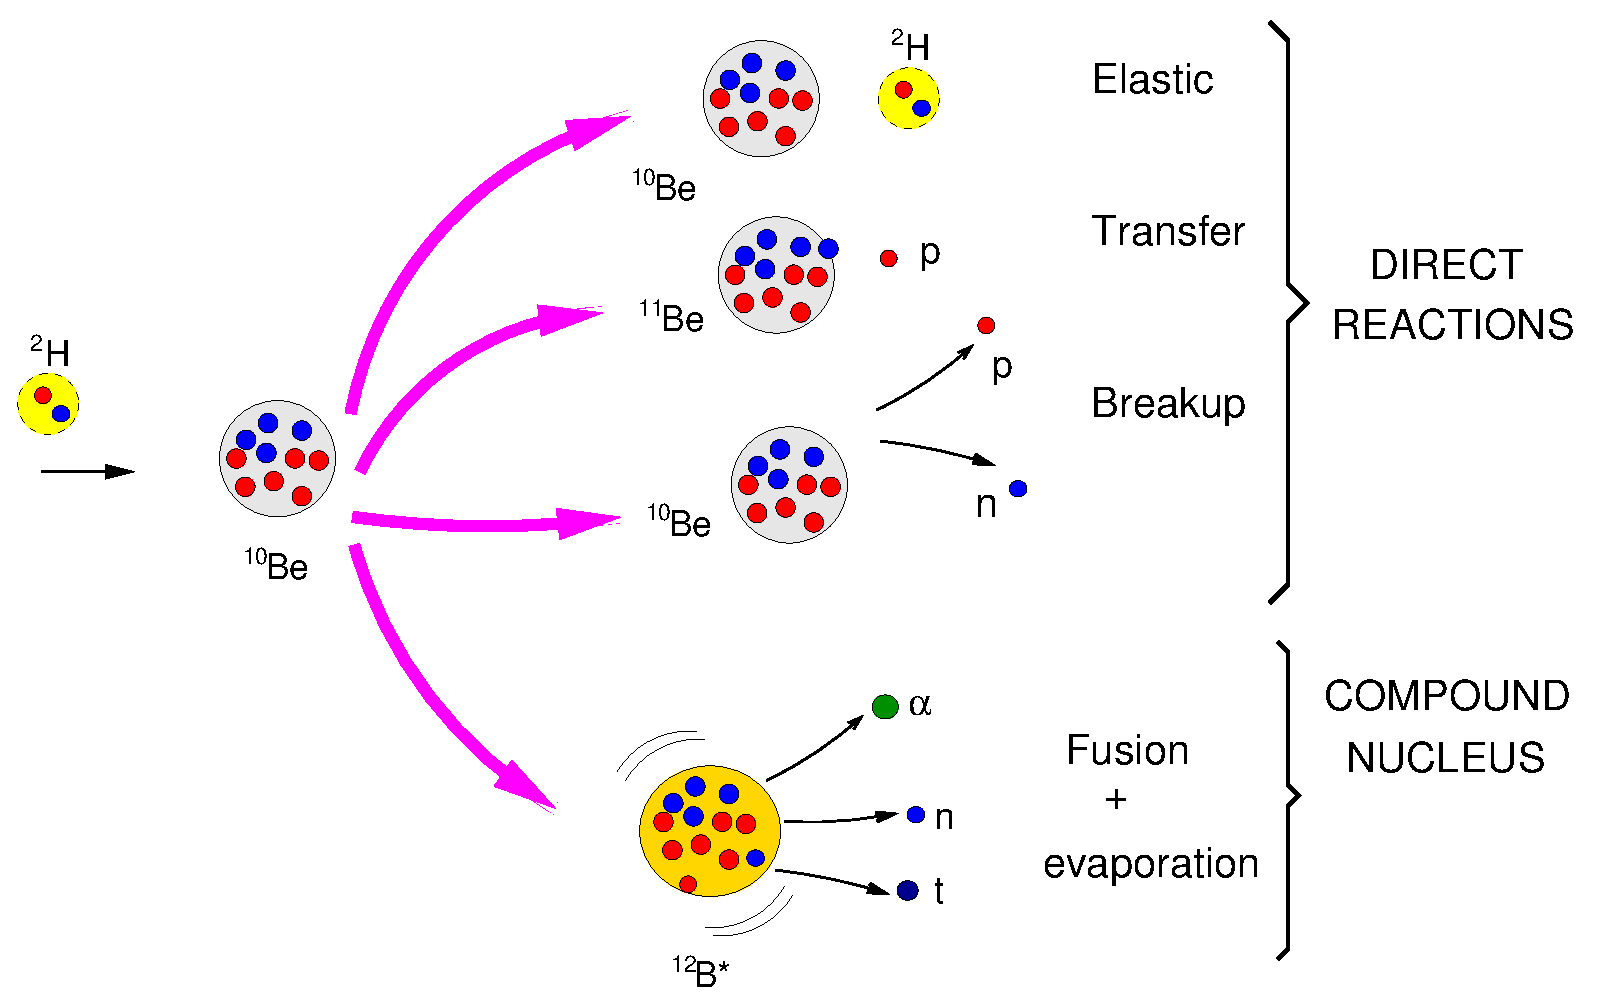
\includegraphics{figs/be10d_chans.eps}} \par}
\end{figure}

\end{frame}





%----------------------------------------
\slide{Direct versus compound reactions}

{\sc \brick Direct:} elastic, inelastic, transfer,\ldots
\begin{itemize}
\setlength{\itemsep}{14pt}
\item ``fast'' collisions (10$^{-21}$~s).
\item only a few modes (degrees of freedom) involved
\item  small momentum transfer
\item angular distribution asymmetric about $\pi/2$ (peaked forward)
\end{itemize}

\vspace{0.5cm}

{\sc \brick Compound:} complete, incomplete fusion.
\begin{itemize}
\setlength{\itemsep}{14pt}
\item many degrees of freedom involved
\item large amount of momentum transfer
\item ``loss of memory''  $\Rightarrow$ almost symmetric distributions forward/backward
\end{itemize}
\end{frame}





%---------------------------------------------------------
\slide{Linking theory with experiments: the cross section}

\let\psgrid\relax
\begin{pspicture}(8,4)
\psgrid
\rput(2,3.0){\rnode{F1}{
\psframebox[fillcolor=red!10,fillstyle=solid,framearc=0.15,linecolor=brick]{
%\psovalbox*[fillcolor=LightBlue,shadow=true]{
 \parbox{3.0cm}{
 \begin{center}
 EXPERIMENT 
 \end{center}

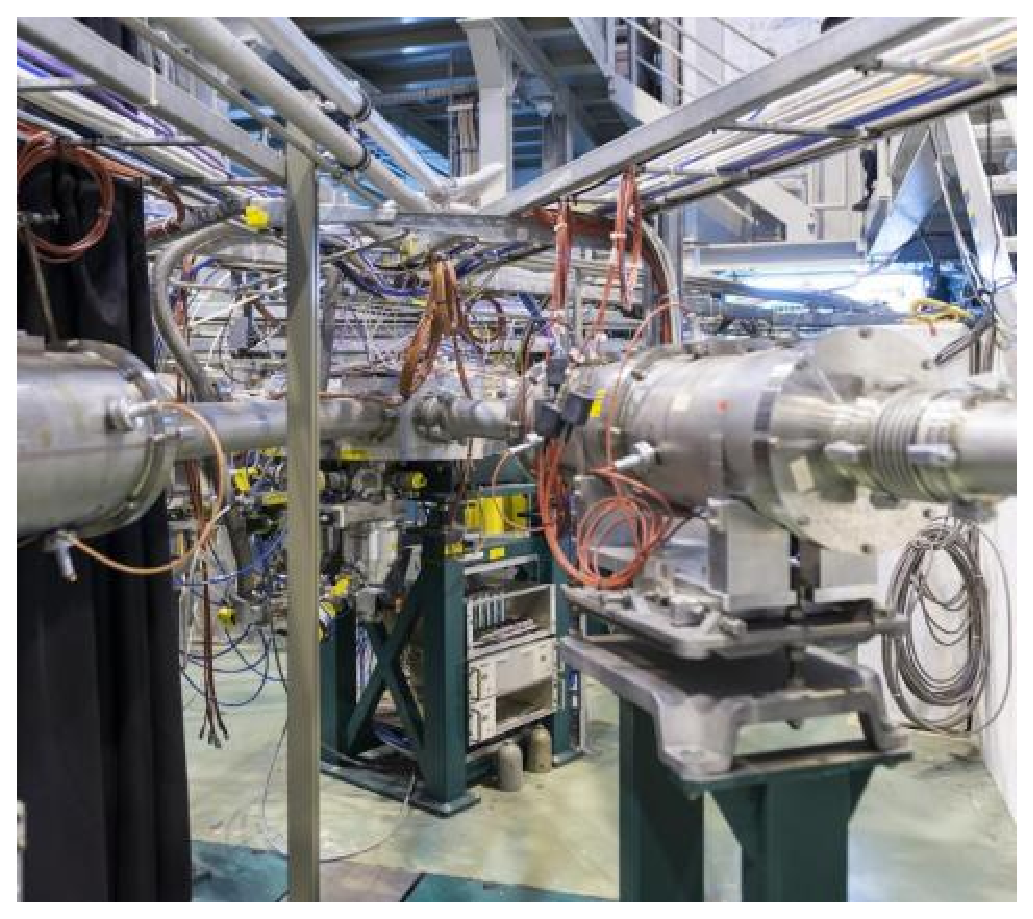
\includegraphics[width=0.25\columnwidth]{figs/isolde.eps}
}%parbox
}}}
\rput(10,3.0){\rnode{F2}{
\psframebox[fillcolor=red!10,fillstyle=solid,framearc=0.15,linecolor=brick]{
%\psovalbox*[fillcolor=LightBlue,shadow=true]{
 \parbox{3.0cm}{
\begin{center} THEORY \\
 ($H \Psi = E \Psi$) 
\end{center}

%  $ \psframebox[fillcolor=green!40,framearc=0.2]{
% H \Psi = E \Psi
% }%psframe
% $

\includegraphics[width=0.22\columnwidth]{figs/computer.eps}
}%parbox
}}}

\pause

\rput(5.5,0.0){\rnode{T1}{\psovalbox*[fillcolor=green!40,shadow=true,fillstyle=solid]{ 
 \parbox{3.0cm}{
CROSS SECTIONS
$$
\frac{d\sigma}{d\Omega}, \frac{d\sigma}{dE}, etc
$$
}
}}}
\end{pspicture}


{\nccurve[linecolor=red,angleA=-90,angleB=180,linewidth=5pt]{->}{F1}{T1}}
{\nccurve[linecolor=red,angleA=-90,angleB=0,linewidth=5pt]{->}{F2}{T1}}
%{\nccurve[linecolor=red,angleA=0,angleB=180]{->}{F3}{T1}}
\end{frame}






\begin{comment}
%---------------------------------------------------------------------------------------
\slide{Experimental cross section}
\begin{itemize}
\item Experimental data consist of cross sections for one or more detected particles

\begin{center}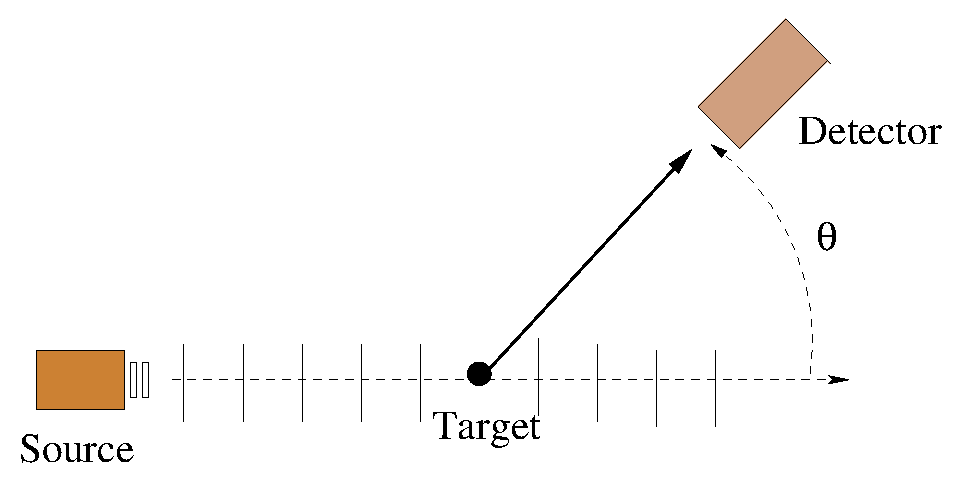
\includegraphics[width=0.35\textwidth]{figs/scattering1.eps}\end{center}

\item Differential cross section:
$$
%\psframebox[fillcolor=green!40,fillstyle=solid,framearc=0.2]{
\psframebox[fillcolor=green!15,linecolor=blue,framearc=0.1,fillstyle=solid]{
\Delta I = I_0 ~ n_t ~ \textcolor{red}{ \frac{d \sigma}{d\Omega} } \Delta \Omega
}%psframe
$$
\begin{itemize}
\item $I_0$: incident particles per unit time
\item $n_t$: number of target nuclei per unit surface
\item $\Delta \Omega$: solid angle of detector
\item $\Delta I$: detected particles per unit time in $\Delta \Omega$
\item $\textcolor{red}{ {d \sigma}/{d\Omega} }$: differential cross section
\end{itemize}
\end{itemize}


\end{frame}
\end{comment}


%---------------------------------------------------------------------------------------
\slide{Experimental cross section}
%\begin{itemize}
%\item Experimental data consist of cross sections for one or more detected particles
\begin{columns}
\column{0.5\textwidth}
\begin{center}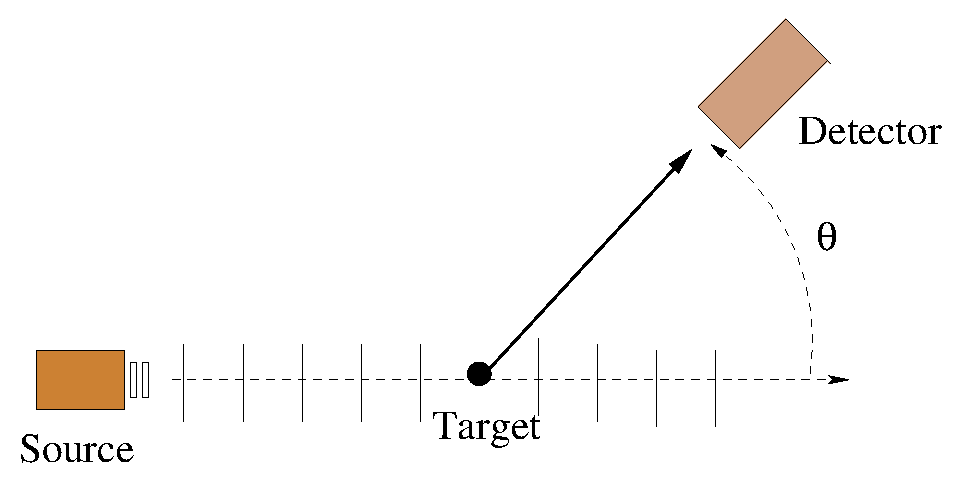
\includegraphics[width=0.8\columnwidth]{figs/scattering1.eps}\end{center}
\column{0.5\textwidth}
$$
%\psframebox[fillcolor=green!40,fillstyle=solid,framearc=0.2]{
\psframebox[fillcolor=green!15,linecolor=blue,framearc=0.1,fillstyle=solid]{
\Delta I = I_0 ~ n_t ~ \textcolor{red}{ \frac{d \sigma}{d\Omega} } \Delta \Omega
}%psframe
$$
\end{columns}

\vspace{0.5cm}
%\item Differential cross section:
% $$
% \psframebox[fillcolor=green!15,linecolor=blue,framearc=0.1,fillstyle=solid]{
% \Delta I = I_0 ~ n_t ~ \textcolor{red}{ \frac{d \sigma}{d\Omega} } \Delta \Omega
% }%psframe
% $$
\begin{itemize}
\item $\Delta I$: detected particles per unit time in $\Delta \Omega$
\item $I_0$: incident particles per unit time
\item $n_t$: number of target nuclei per unit surface
\item $\Delta \Omega$: solid angle of detector
\item $\textcolor{red}{ {d \sigma}/{d\Omega} }$: differential cross section
\end{itemize}
%\end{itemize}

$$
\psframebox[fillcolor=green!15,linecolor=blue,framearc=0.1,fillstyle=solid]{
\frac{d\sigma}{d\Omega} =  \frac{\textrm{flux of scattered particles through $dA= r^2 d\Omega$} }{ \textrm{incident flux} }
}%psframe
$$

\end{frame}






%----------------------------------------------------------------
\slide{Projectile and target internal Hamiltonians}
\begin{itemize}
\item Mass partitions: $\alpha$, $\beta$,$\ldots$
\item {\brick Internal} proj. + target Hamiltonians: $H_\alpha(\xi_\alpha) \equiv H_p(\xi_p) + H_t (\xi_t)$
\item Internal states:
$
[H_\alpha (\xi_\alpha) - \varepsilon_\alpha] \Phi_\alpha (\xi_\alpha)=0 \quad \{\varepsilon_\alpha\}=\textrm{excitation energies}
$
\item Different mass partitions  have different Hamiltonians: $H_\alpha(\xi_\alpha)$,$H_\beta (\xi_\beta)$, etc
\end{itemize}

\resizebox*{0.7\textwidth}{!}{\input{figs/be10d_chans_H.pstex_t}}
%\scalebox{.4}{ \input{figs/be10d_chans_H.pstex_t} }
\end{frame}




%----------------------------------------------
\slide{Model Hamiltonian and model wavefunction}

\begin{block}{Full Hamiltonian}
$$
\psframebox[linecolor=red,framearc=0.1,framesep=5pt]{
H= \hat{T}_\bR + H_p(\xi_p) + H_t(\xi_t) + V(\bR,\xi_p,\xi_t) 
}%psfr
$$
\begin{itemize}
\item $\hat{T}_\bR $: proj.--target kinetic energy
\item $H_p(\xi_p)$: projectile Hamiltonian
\item $H_t(\xi_t)$: target Hamiltonian
\item $V(\bR,\xi_p,\xi_t)$: projectile--target interaction
\end{itemize}
\end{block}

%\begin{block}{Scattering wavefunction}
Time-independent Schrodinger equation:
$$
\psframebox[linecolor=red,framearc=0.1,framesep=5pt]{
[H - E ] \Psi(\bR,\xi_p,\xi_t) = 0
}%psfr
$$
%\end{block}

\end{frame}





%------------------------------------------------------
\slide{Scattering wavefunction}

\begin{center}
%\begin{figure}
\begin{minipage}{0.62\textwidth}
\includegraphics[width=0.75\columnwidth]{figs/scattering.eps}
\end{minipage}
\begin{minipage}{0.35\textwidth}
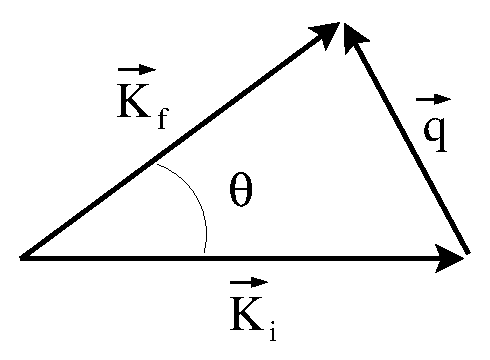
\includegraphics[width=0.6\columnwidth]{figs/transfer_mom.eps}
\end{minipage}
%\caption{\label{fig:scattering} Left: schematic representation of a scattering process. Right: initial, final and transferred momenta.}
%\end{figure}
\end{center}

%\includegraphics[width=0.5\columnwidth]{figs/scattering.eps}


Among the many mathematical solutions of $ [H - E ] \Psi = 0$ we are interested  in those behaving asymptotically as:

%\parbox{0.9\textwidth}{
$$
%\psframebox[fillcolor=magenta!10,linecolor=red,framearc=0.1,fillstyle=solid,framesep=8pt]{
\psframebox[linecolor=red,fillcolor=orange!10,fillstyle=solid,framearc=0.2,framesep=8pt]{
\Psi^\mathrm{(+)}_{\bK_\alpha} \rightarrow   \Phi_\alpha(\xi_\alpha) e^{i \bK_\alpha \cdot \bR_\alpha} +
 \textrm{(outgoing spherical waves in $\alpha$, $\beta$, $\ldots$)}
}%psframebox
$$
%}%parbox
%}%psframe


%\end{itemize}


\end{frame}


%-----------------------------------------------
\slide{Scattering amplitude and cross sections}

%\begin{center}
%\psframebox[fillcolor=magenta!5,linecolor=red,framearc=0.1,fillstyle=solid,framesep=-8pt]{
\psframebox[linecolor=red,fillcolor=orange!10,fillstyle=solid,framearc=0.2,framesep=-8pt]{
\parbox{0.9\textwidth}{
\begin{align*}
\Psi^\mathrm{(+)}_{\bK_\alpha}   \xrightarrow{R_\alpha \gg}  & \Phi_\alpha(\xi_\alpha) e^{i \bK_\alpha \cdot \bR_\alpha} +  \Phi_\alpha(\xi_\alpha) f_{\alpha,\alpha}(\theta) \frac{e^{i K_\alpha R_\alpha}}{R_\alpha}  & \quad \textrm{(elastic)}
\\
  & +\sum_{\alpha' \neq \alpha} \Phi_{\alpha'}(\xi_\alpha) f_{\alpha',\alpha}(\theta) \frac{e^{i K_{\alpha'} R_\alpha}}{R_\alpha} 
 & \quad \textrm{(inelastic)}
 \\
\Psi^\mathrm{(+)}_{\bK_\alpha}   \xrightarrow{R_\beta \gg}  & \sum_{\beta} \Phi_\beta(\xi_\beta) f_{\beta,\alpha}(\theta) \frac{e^{i K_\beta R_\beta}}{R_\beta} 
 & \quad \textrm{(transfer)}
\end{align*}
}%parbox
}%psframe

\vspace{0.5cm}


%\begin{block}{Cross sections:}
{\bf Cross sections:} 
$$
%\psframebox[fillcolor=magenta!8,linecolor=red,framearc=0.1,fillstyle=solid,framesep=6pt]{
\psframebox[linecolor=red,fillcolor=orange!10,fillstyle=solid,framearc=0.2,framesep=6pt]{
\left ( \frac{d\sigma}{d\Omega} \right)_{\alpha \rightarrow \beta} = \frac{K_\beta}{K_\alpha} \left| f_{\beta,\alpha}(\theta) \right|^2 
}%psr
\quad
E= \frac{\hbar^2 K^2_\alpha}{2 \mu_\alpha} + \varepsilon_\alpha = \frac{\hbar^2 K^2_\beta}{2 \mu_\beta} + \varepsilon_\beta
$$ 
%\end{block}
 {\red $f_{\beta,\alpha}$ } is called {\brick scattering amplitude}

%
\end{frame}

%---------------------------------------------------------
\slide{}
{\bf Ideally, the strategy would be:}
\begin{enumerate}
\item Choose structure model for $H_\alpha(\xi)$
\item Compute $\Psi^\mathrm{(+)}$ by solving $[H-E]\Psi^{(+)}=0$
\item Consider the limit $R \gg$ of $\Psi^\mathrm{(+)}$ 
\item Project it on the desired final state to extract the scattering amplitude:
$$
(\Phi_{\alpha'}(\xi_\alpha) | \Psi^\mathrm{(+)} \rangle = {\red f_{\alpha',\alpha}(\theta)} \frac{e^{i K_{\alpha'} R_\alpha}}{R_\alpha} 
$$ 
\end{enumerate}

\pause
{\bf But...}
\begin{itemize}
\item $\Psi$ is a solution of a complicated many-body problem, not solvable in most cases. 
\item The number of accesible channels and states can be huge. 
\end{itemize} 

\vspace{0.5cm}

\ding{233}{\it So, in practice, we will be happy with an approximation of {\red $\Psi$} (or ${\red f(\theta)}$) in a restricted modelspace} 
\end{frame}

%---------------------------------------------------------





\subsection{Feshbach formalism: P and Q spaces}
%---------------------------------------------------------
\slide{Defining our model space: Feshbach formalism}

\begin{itemize}
\item Divide the full space into two groups: \textcolor{red}{P} and {\red Q}
\begin{itemize}
\item[\ding{233}] {\red P}: channels of interest
\item[\ding{233}] {\red Q}: remaining channels 
 \end{itemize}

\item  Write $\Psi = \Psi_P + \Psi_Q$

\begin{center}
%\psframebox[fillcolor=magenta!5,linecolor=red,framearc=0.1,fillstyle=solid,framesep=-7pt]{
\psframebox[linecolor=red,fillcolor=orange!10,fillstyle=solid,framearc=0.2,framesep=-7pt]{
\parbox{0.4\textwidth}{
\begin{align*}
(E-H_{PP}) \Psi_P & = H_{PQ} \Psi_Q  \\
(E-H_{QQ}) \Psi_Q & = H_{QP} \Psi_P 
\end{align*}
}%parbox
}%psframe
\quad ( $H_{PP}=P H P $,  $H_{PQ}=P H Q $,  etc )
\end{center}

\item Eliminate (formally) $\Psi_Q$:
$$
%\psframebox[fillcolor=magenta!5,linecolor=red,framearc=0.1,fillstyle=solid,framesep=5pt]{
\psframebox[linecolor=red,fillcolor=orange!10,fillstyle=solid,framearc=0.2,framesep=5pt]{
\underbrace{ \left [H_{PP} + H_{PQ} \frac{1}{E- H_{QQ} + i \epsilon} H_{QP}  \right ] }_{H_\mathrm{eff} } \Psi_P = E \Psi_P 
}%psframe
$$

\item $H_\mathrm{eff}$ too complicated (complex, energy dependent, non-local) $\Rightarrow$  needs to be replaced by a simpler Hamiltonian: 
$$
H_\mathrm{eff} \longrightarrow H_\mathrm{model} \quad \textrm{(complex, energy dependent)}
$$ 

\end{itemize}
\end{frame}


%-------------------------------------------
\slide{Strategy for reaction calculaions}

We need to make a choice for:
\bigskip

\begin{enumerate}
\setlength{\itemsep}{14pt}
\item {\brick Modelspace:} what channels are to be included?

\item {\brick Structure model:} for projectile and target
\item[] (Microscopic, collective, cluster...)

\item {\brick Reaction formalism}

\end{enumerate}

\end{frame}


%---------------------------------------
\subsection{Defining the modelspace}
\slide{Choice of the modespace: the d+\nuc{10}{Be} example}

\begin{figure}{\par \resizebox*{0.7\textwidth}{!}
{\includegraphics{figs/be10dp_channels.eps}} \par}
\end{figure}

\end{frame}




%------------------------------------------------------
\slide{Choice of structure model: from the many-body problem to the few-body picture}

\scriptsize
\begin{center}
\begin{pspicture}(10,6)
%\psgrid

\visible<1->{
 % --------------------------- MIC CORE ------------------------------------- %  
\rput(4,6){
   \psframebox[linewidth=0,shadow=true,fillcolor=green!25,fillstyle=solid]{%
    \scriptsize Microscopic models 
   }%psframe
   }%rput

\rput(1,5){
  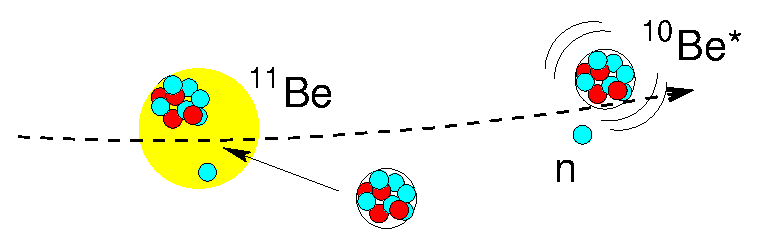
\includegraphics[height=1.25cm]{\images/be11t_mic.eps} 
   }%rput    

\rput(8,5){
   \parbox{0.8\columnwidth}{
    \begin{itemize}    
%    \item[\ding{52}] Achieved for 2-body (CDCC) 
    \item[\ding{52}] Fragments described microscopically
    \item[\ding{52}] Realistic NN interactions (Pauli properly accounted for) 
    \item[\ding{54}] Numerically demanding / not simple interpretation.

    \end{itemize}
    }%parbox
    }%rput
}%visible

 % --------------------------- INERT CORE ------------------------------------- %  
\visible<2->{
\psline[linecolor=orange!40,linewidth=4pt]{<->}(10.7,0)(10.7,6.0)
\rput{-90}(11.,1.5){Few-body}
\rput{-90}(11.,5.0){Many-body}

\rput(4,1.3){
   \psframebox[linewidth=0,framearc=0.2,shadow=true,fillcolor=green!25,fillstyle=solid]{
    Inert cluster models
   }%psframe
   }%rput

\rput(8,0.1){
   \parbox{0.8\columnwidth}{
    \begin{itemize}
%    \item[\ding{54}] Ignores core-excitation admixtures and core transitions.
    \item[\ding{54}] Ignores cluster excitations (only few-body d.o.f).
    \item[\ding{54}] Phenomenological inter-cluster interactions (aprox.~Pauli). 
    \item[\ding{52}] Exactly solvable (in some cases).
    \item[\ding{52}] Achieved for 3-body and 4-body (eg.~coupled-channels, Faddeev).
    \end{itemize}
    }%parbox
    }%rput

\rput(1,0.2){
  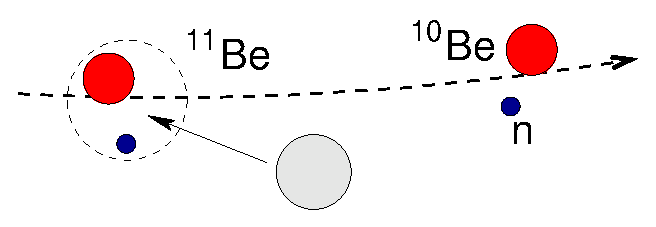
\includegraphics[height=1.25cm]{\images/be11t_inert.eps} 
   }%rput    
}%visible

\visible<3->{
 % --------------------------- CORE EXC ----------------------------------------- % 
\rput(4,3.6){
   \psframebox[linewidth=0,framearc=0.2,shadow=true,fillcolor=green!25,fillstyle=solid]{
    \scriptsize Non-inert-core few-body models   
   }%psframe
   }%rput

\rput(1,2.6){
  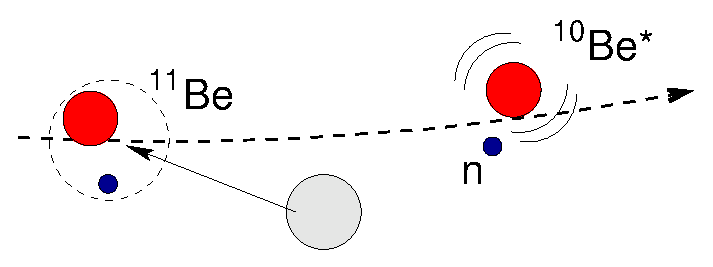
\includegraphics[height=1.25cm]{\images/be11t_corex.eps} 
   }%rput    

\rput(8,2.6){
   \parbox{0.8\columnwidth}{
    \begin{itemize}    
    \item[\ding{52}] Few-body + some relevant collective d.o.f. 
%    \item[\ding{52}] Core excitation within collective model.
    \item[\ding{52}] Pauli approximately accounted for.
    \item[\ding{52}] Achieved for 3-body problems (coupled-channels, Faddeev).    
    \end{itemize}
    }%parbox
    }%rput

}%visible

\end{pspicture}
\end{center}

\end{frame}

\endinput




%-----------------------------------------------------------------------------------------
\slide{}
\begin{center}
\psframebox[fillcolor=green!10,linecolor=blue,framearc=0.1,fillstyle=solid,framesep=5pt]{
Inert-core models: the CDCC method example
}%psframe
\end{center} 
\end{frame}


%%%%%%%%%%%%%%%%%%%%%%%%%%%%%%%%%%%%%%%%%%%%%%%%%%%%%%%%%%%%%%%%%%%%%%%%%%%%%%%%%%%%%%%%%%%%%%%%%%%%%%%%%%%%%%%%%%%%


%---------------------------------------------------------
\slide{Linking theory with experiments: the cross section}


\visible<1>{
\rnode{F1}{
\rput(0.2\columnwidth,0.35\textheight){
\psframebox[fillcolor=red!10,fillstyle=solid,framearc=0.15]{
 \parbox{5cm}{
{\blue \scriptsize \centering EXPERIMENT}
 \begin{center}{\brick \scriptsize Eg:~Spectroscopic factors \\ (knockout vs transfer reactions)} 
 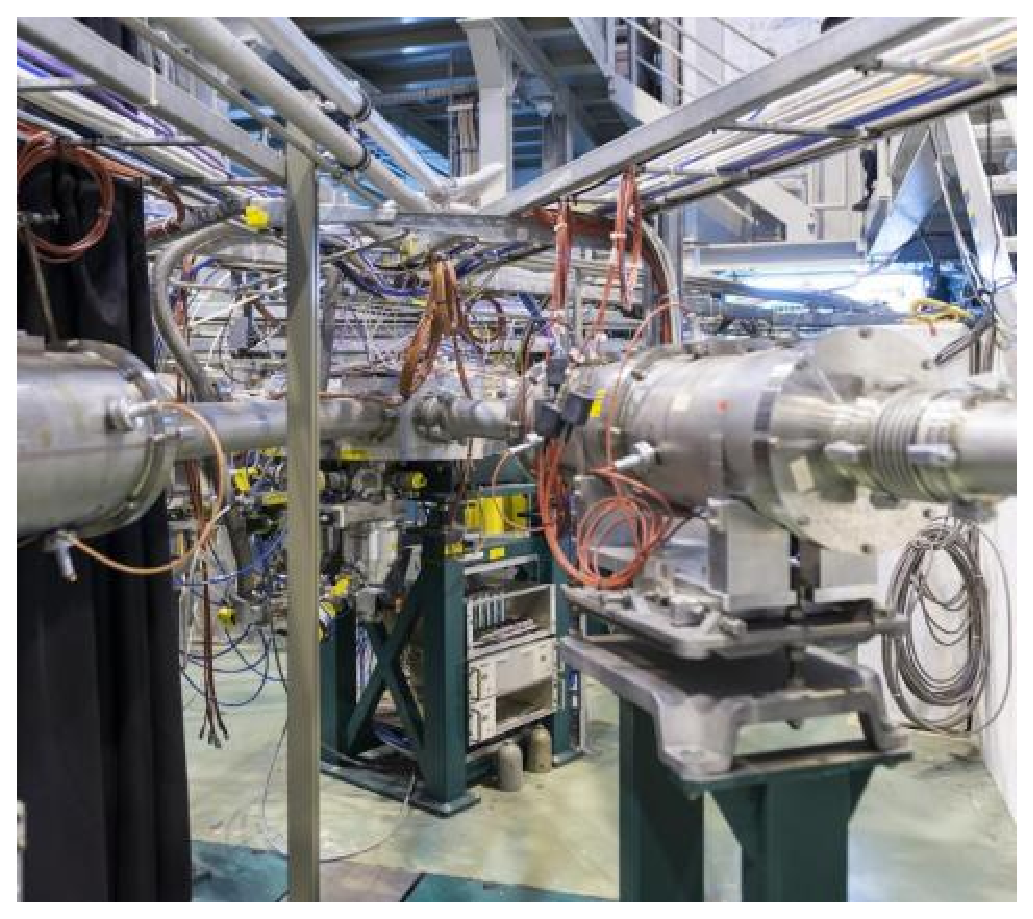
\includegraphics[width=3.0cm,framearc=0.2]{figs/isolde.eps} \\
 \end{center}
  }%parbox
 }%psframe
}%rput
}%rnode
}%visible

\end{frame}



\slide{}
\begin{picture}(0,0)%
\includegraphics{figs/be10d_chans_H.pstex}%
\end{picture}%
\setlength{\unitlength}{3947sp}%
%
\begingroup\makeatletter\ifx\SetFigFont\undefined%
\gdef\SetFigFont#1#2#3#4#5{%
  \reset@font\fontsize{#1}{#2pt}%
  \fontfamily{#3}\fontseries{#4}\fontshape{#5}%
  \selectfont}%
\fi\endgroup%
\begin{picture}(9040,5643)(247,-5589)
\end{picture}%

\end{frame}




\slide{}
\let\psgrid\relax
\begin{pspicture}(8,4)
\psgrid
\rput(1,1){\rnode{F1}{\psovalbox*[fillcolor=LightBlue,shadow=true]{Deformation}}}
\rput(1,1.5){+}
\rput(1,2.2){\rnode{F2}{\psovalbox*[fillcolor=LightBlue,shadow=true]{Pairing}}}
\rput(1,2.8){+}
\rput(1,3.4){\rnode{F3}{\psovalbox*[fillcolor=LightBlue,shadow=true]{Weak binding}}}

\rput(7.5,2.2){\rnode{T1}{\psovalbox*[fillcolor=green!40,shadow=true,fillstyle=solid]{ 
 \parbox{5cm}{
\begin{itemize}
\small
\item How to combine them consistently in {\bf structure}?  
\item How do these effects show  up  in {\bf reactions}?
\end{itemize}
}
}}}
\end{pspicture}

{\nccurve[linecolor=red,angleA=0,angleB=180]{->}{F1}{T1}}
{\nccurve[linecolor=red,angleA=0,angleB=180]{->}{F2}{T1}}
{\nccurve[linecolor=red,angleA=0,angleB=180]{->}{F3}{T1}}
\end{frame}




